\section{Speech Synthesis History}\label{ssh}
One of the earliest successful attempts to produce speech synthesis were made over two hundred years ago (Flanagan 1972) in 1779 by Professor Kratzensteint, who build some apparatus that represented the human vocal tract to produce five long vowels due to the physiological differences between the vowels. The apparatus were acoustic resonators similar to the human vocal tract and he activated them with reeds like the one used in musical instruments.\\
The first recorded success in connected speech synthesis was achieved by  Wolfgang von Kempelen in 1791 when he completed the construction of his "Acoustic-Mechanical Speech Machine" which was a ingenious pneumatic synthesizer (see figure \ref{kempelen}).
\begin{figure}[!htb]
	\begin{center}
	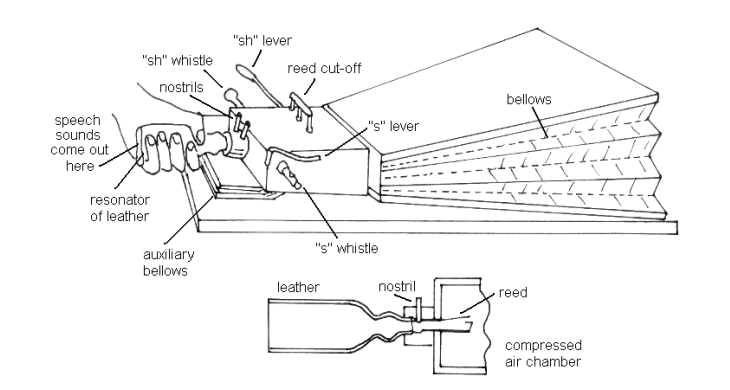
\includegraphics[width=1\textwidth]{img/kempelen.png}
	\end{center}
	\caption{\label{kempelen}Kempelen Acoustic-Mechanical Speech Machine \ref{donde saque la imagen}}
\end{figure}
The machine had a pressure chamber for the lungs, a vibrating reed to act as vocal cords and a leather bag fir the vocal tract action. Changing the shape (by hand) of the leather bag different vowel sounds were produced. Constants were simulated by four separate constricted passages that were controlled by the fingers. There were also a couple of hiss whistles to allow the simulation of fricatives and a pair of openings to simulate the nostrils. For plosive sounds a model of a vocal tract that included a hinged tongue and movable lips was employed. To produce a sequence of sounds that seems like speech a lot of practice was needed.\\
En el de acoustic pone que la imagen fue de una reproduccion mas complicada que hizo alguien despues...\\
The connection between a specific vowel sound and the geometry of the vocal tract was found in 1838 by Willis, who synthesized different vowels with tube resonators and discovered that the quality of the vowel depended only on the length of the tube and not on its diameter.
Also in the late 1800's Alexander Graham Bell constructed with his father same kind of speaking machine as the Wheastone's speaking machine that was a reproduction of the Kempelen speaking machine with a few changes.\\
With the 20th century came the development of electronics and later of electronic resonators. There were a few attempts early in the century to use electronic resonators in such a way that they could produce steady state vowels. An example of this is the electrical synthesis device created by Stewart in 1922. The synthesizer had a buzzer as excitation and two resonant circuits to model the acoustic resonances of the vocal tract. The machine was able to generate single static vowels sounds with two lowest formants, but not any consonants or connected utterances. Obata and Teshima discovered the third formant in vowels. With the three firs formants is enough for intelligible synthetic speech. It was finally in the late 1930's when the work of Homer Dudley at the Bell Laboratories produced the first electrical connected speech synthesizer.\\
Dudley developed two devices. One of them, the 'Voder' (figure \ref{voder}) was basically a parallel array if ten electronic resonators arranged as contiguous band-pass filters spanning  the important frequencies of the speech spectrum. It consisted of a wrist bar for selecting a voicing or noise source and a foot pedal to control the fundamental frequency. The source signal was routed through ten band-pass filters whose output gain were controlled via keyboard. A considerable skill was needed to play a sentence on the device and the quality was far from good, so it was consider of little practical value, but after the demonstration of the Voder the scientific world became more and more interested in speech synthesis.\\
\begin{figure}[!htb]
	\begin{center}
	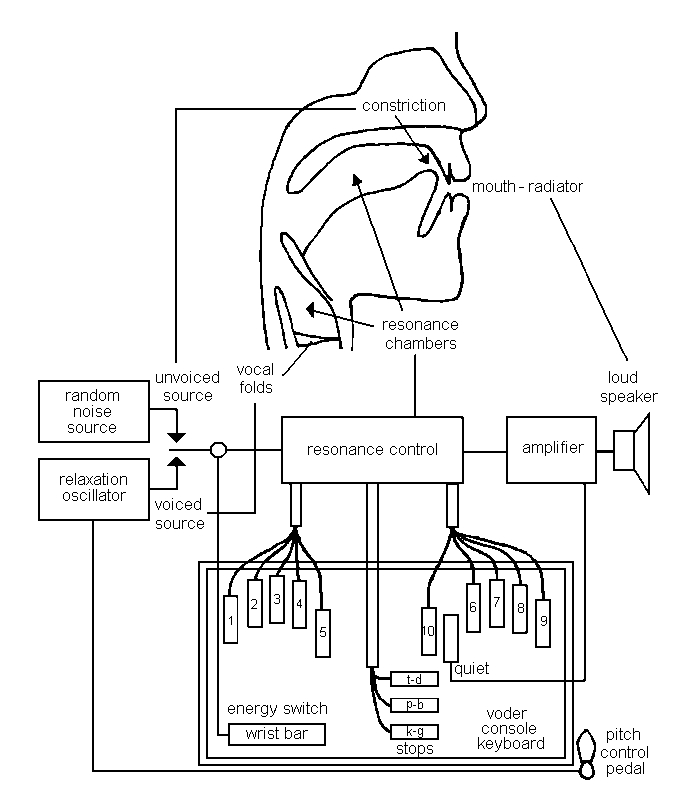
\includegraphics[width=1\textwidth]{img/voder.png}
	\end{center}
	\caption{\label{voder}Dudley's Voder speech synthesizer \ref{de donde la saque}}
\end{figure}
The other device Dudley made was called a 'channel vocoder'. This channel vocoder and all subsequent vocoders are basically analysis/synthesis devices. They are divided into two halves, an analysis half and a synthesis half. The fist one analyses an incoming speech signal and obtains certain parameters from that natural signal. This parameters are passed as codes to the second half (synthesis) and there they are used to resynthesize a synthetic version of the incoming speech. The channel vocoder is the simplest of the vocoders. It is divided in two branches, one of them determines if the signal is voice or unvoiced and if it voiced it determines the pitch. This information is used to produce a synthetic source. The other branch is a bank of electronic resonators acting like band-pass filters which measure the level of the signal in each frequency band at each point in time. With this information the synthetic source is produced (in the synthesis half of the vocoder) and is mixed with a spectral envelope reconstituted from the filter level values to produce synthetic version of the original signal.\\
The vocoders were originally developed at the Bell Telephone Labs as devices which allowed a signal to be coded more efficiently and thus allowed more conversations at the same time in the telephone network. More other vocoder configurations have been developed with simply filter banks and rely on complex mathematical transforms of the data (e.g Linear Prediction Coefficient (LPC) vocoders) or on the detection of the formants in the speech signal.\\
In 1951 the pattern play-back machine (figure \ref{spectro}) was developed by Cooper, Liberman and Borst. It reconverted recorded spectrogram patters into sounds, either original or modified form.\\
\begin{figure}[!htb]
	\begin{center}
	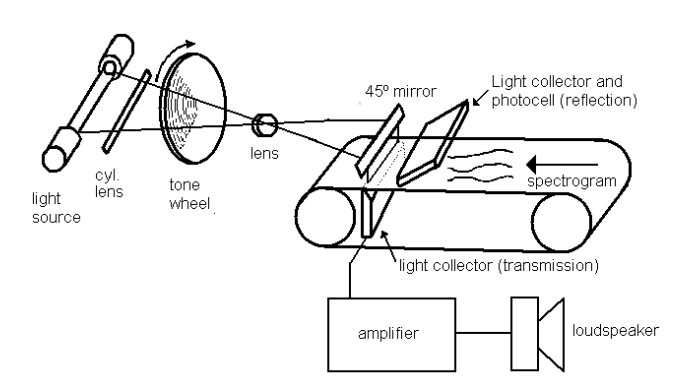
\includegraphics[width=1\textwidth]{img/spectrogram.png}
	\end{center}
	\caption{\label{spectro}Pattern play-back machine \ref{de donde la saque}}
\end{figure}
In 1953 Walter Lawrence introduced the first formant synthesizer, PAT, which looked similar to the pattern playback. It consisted if three electronic formant resonator connected in parallel and the input signal was either a buzz or noise. A moving glass slide was used to convert painted patterns into six time functions to control the three formant frequencies, voicing amplitude, fundamental frequency and noise amplitude. At that time Gunnar Fant introduced the first cascade formant synthesizer OVE I wich consisted of formant resonators connected in cascade. Ten years later he introduced an improve, OVE II, with Martony which consisted on separated parts to model the transfer function of the vocal tract for vowels, nasal, and obstruent consonants.\\
In 1958 the first articulatory synthesizer (The DAVO) was introduced at the Massachusetts Institute of Technology by George Rosen. In mid 1960's the first experiments with Linear Predictive Coding (LPC) were made, but it was first used in low-cost systems and its quality was poor. With some modifications this method has been found very useful.\\
In 1979 Allen, Hunnicutt and Klatt demostrated the MITalk laboratory text to speech system. Two years later Klatt introduced his Klattalk system, which used a new sophisticated voicing source.\\
The first reading aid for blind people with an optical scanner was introduced in 1976 by Kurzweil. This system was capable to read quite well multiform written text.\\
In the late 1970's a lot of commercial TTS and speech synthesis products were introduced. The first integrated circuit was probably the Votrax chip which consisted of cascade formant synthesizer and simple low-pass smoothing circuits. In 1980 The Linear Prediction Coding (LPC) based Speak-n-Spell synthesizer based on low cost linear prediction synthesis chip was introduced by Texas Instruments and it was used for an electronic reading aid for children.\\
Modern speech synthesis technologies involve quite complicated and sophisticated methods and algorithms. One of the methods applied "recently" in speech synthesis is Hidden Markov Models (HMM, section \ref{hmm}).